\documentclass[a4paper,10pt,twocolumn,uplatex]{jsarticle}
\usepackage{style/nislab}

%---------------------------------------------------------------------
% レジュメ種別・日付設定(要変更)
% \type{} 1:修士論文諮問会 2:卒業論文発表会 else:月例発表会
\type{3}
\year{2021}
\month{4}
\date{1}

%---------------------------------------------------------------------
% ページ番号設定(要変更)
\setcounter{page}{1}

%---------------------------------------------------------------------
\begin{document}
%---------------------------------------------------------------------
% タイトル作成部分(要変更)
% \maketitle{タイトル}{title}{名前}{name}
\maketitle{タイトルタイトルタイトルタイトルタイトルタイトル}
{Title Title Title Title Title Title}
{竹内 一真}
{Kazuma Takeuchi}

%---------------------------------------------------------------------
\section{はじめに}
近年,多方面でのドローンを活用した事業が進出しており,屋内での小型ドローンの利用も期待されている.しかし,狭小空間でのドローンの飛行は,障害物が多く,操縦者から見えない場所であったりと,遮られた視点からの操縦を必要とし,操縦は困難が懸念される.
\par
カメラ搭載のドローンを使用する場合では,操縦者はドローンから送られてくる映像を元に操縦が可能となる.そのような操縦方法によって,安全な距離から狭小空間を探索することができるが,カメラが前方しか写さないという点からFPV(一人称視点)の操縦では前方以外の死角が多くなり,また,機体の大きさを掴めないという欠点がある.
\par
そこで,拡張現実を用いることで,操縦者の死角領域内を可視化し,狭小空間での操縦性の向上を図れると考えられる.また,操縦者視点の操縦を実現する上で,障害物までの距離感が掴めないことが懸念されている.自律飛行のドローンでの障害物回避に関する研究は数多くされているが,操縦者にどのように障害物を知覚させるかの研究はされていない.そこで,ドローン近傍の障害物を検知するデザイン案を提案することで,操縦者にとってどのような情報が障害物までの距離感を掴むのに適しているかを検討した.
これにより操縦者に継続的な空間認識を確保しつつ,操縦性を向上させる手法を提案します.

%---------------------------------------------------------------------
\section{図表のベストプラクティス}
\LaTeX{}を使いこなすにあたり,図表の活用は重要である.基本的にはLaTex Wiki\cite{latex_wiki}を参考にすれば問題ない.\par
\section{関連研究}
\subsection{}
Eratらの研究では\cite{drone},狭い場所でのドローン操縦が困難ということで,三人称視点のドローン操縦手法を提案している.ドローンがSLAM技術で空間マッピングをすることで,空間の仮想現実を構築し,閉鎖環境をみえるようにするというものである.しかし,空間の環境は事前に準備されたものであり,動的に再構築することがないので利便さに欠ける.
\subsection{概要}
またMichaelらは\cite{interface},人間がドローンの動きの意図を視覚的に理解するため,ARを用いたユーザインタフェースデザインを作成し評価した.結果として,ドローンに対しARを用いた様々なデザインは,ARなしと比べ,課されたタスク効率を大幅に向上させ,ARを用いることでドローンの操縦性を向上させるための直感的で視覚的な合図を提供することが可能であることが示された.

%---------------------------------------------------------------------
\subsection{図}
図を挿入する場合は,図\ref{fig:sample1}や\figref{fig:sample2}のように引用することができる.図の横幅が大きい場合は,\figref{fig:sample2}のようにすることもできる.\par
ちなみに,\LaTeX{}ではベクターファイルとしてEPSファイルを推奨していた頃もあったようだが,現在はPDFファイルを使用することが推奨されている.PDFファイルに出力するのが前提なら,dvipdfmxではPDF,PNG,JPEG がそのまま使用できる.dvipdfmxはEPSファイルそのものを自分で扱えないので,Ghostscriptを内部で呼び出して変換する.PDFファイルで問題がなければEPSにこだわる必要はないと思われる.ただし,ジャーナルによっては図としてPDFを使うのがダメだったりするので慎重に.

\begin{figure}[!tb]
  \centering
  
\includegraphics[width=\linewidth]{img/sample1.pdf}
  \caption{悩む男の子}
  \label{fig:sample1}
\end{figure}

\begin{figure*}[!tb]
  \centering
  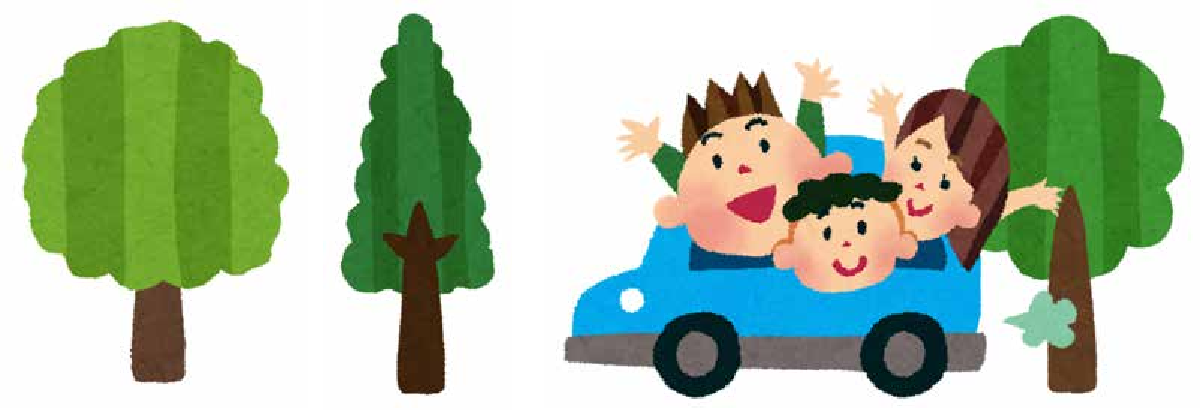
\includegraphics[width=\linewidth]{img/sample2.pdf}
  \caption{ドライブする家族}
  \label{fig:sample2}
\end{figure*}

%---------------------------------------------------------------------

\section{提案手法}\label{discussion}
\subsection{概要}
本研究では,操縦者とドローンの間に障害物があり,ドローンを視認できない環境を想定する.障害物が存在すると判断した際,その障害物を透過することで,操縦者への死角領域の空間認識を提供する.
また,死角領域内をドローンが飛行している際に,近傍の障害物までの距離が掴めない問題点を解決するために,2つのARインタフェースデザインを提案した.

\subsection{Stereo}
Stereoのデザインは,ステレオビジョンを参考にして,ドローンから障害物までの距離に応じて,障害物の色を分けている.Stereoは,全体的な環境の理解を提供しており,ドローン周辺の障害物全ての衝突の危険性を示す.

\subsection{Marker}
Markerのデザインは,ドローンから見て最も近い障害物に対して,目印を付けている.Stereoでは障害物全てが色分けされているため,操縦者を混乱させる可能性がある.Markerでは,最も危険な障害物だけを知覚させるため,Stereoに比べ簡易的なアプローチとなっている.

%---------------------------------------------------------------------

\section{評価}\label{experiment}
\subsection{実装}
提案手法のシステム構成を図2に示す.
実際に使用したドローンはTello EDUであり,操作端末はMacBookProを用いる.ドローン未経験者と経験者による差を出さないために,ドローンの速度,一度に進む距離,旋回角度などは事前に設定してある.
\par
ARHMDはMicrosoft HoloLens2を使用する.
事前にHoloLensのSpatial Mappingにより環境マッピングを行い,静的な3次元環境地図を作成する.ゲーム・アニメーションエンジンであるUnity内の3D仮想空間上でこの3次元環境地図とドローンを現実と同様の配置を行い,操縦者とUnity内の操縦者の位置合わせを行っている.
\par
Stereo,Markerでは共に障害物までの距離によって,危険度を色で示している.Stereoでは,障害物までの距離が0.5mまでを赤色で示し,0.5m~0.7mまでを黄色で示し,0.7m~1.0mまでを緑色で示している.Markerでは障害物までの距離が0.3m~0.5mの際に赤色のマーカーで示し,0.5m~0.7mの際に黄色のマーカーを示す.各デザインの色の使い分けにより,操縦者への資格的支援を行う.

%---------------------------------------------------------------------
\section{まとめと今後の課題}
小型ドローンでの遮られた視点からの狭小空間での操縦は死角の多さや,ドローンと障害物までの距離感が測れないことが懸念され,本研究では操縦者の死角領域内に存在するドローンと周辺を可視化し,ドローン周辺の障害物を知覚するためのARデザインを提案し,実験を行うことで遮られた視点からの狭小空間でのドローン操縦性を評価した.結果として,ARを利用した手法では実験環境での操縦時間が短く,衝突回数も少なかったことから操縦性の向上が確認された.
また,障害物を知覚するためのARデザインでは,ドローン周辺の障害物に危険度を振り分けている手法が,操縦者への操縦への安心を与え,操縦性を向上させたことが確認できた.

%---------------------------------------------------------------------


% \subsection{表}
% 表は\tabref{tab:data_type}のように引用することができ,表を作成する場合は罫線を少なくすることと,横線のみの使用を心がけることが推奨される.

% \begin{table}[!bt]
%   \caption{代表的なデータの型}
%   \label{tab:data_type}
%   \centering
%   \begin{tabular}{lcr}
%     \hline
%     データの型         & 宣言   & ビット幅 \\
%     \hline \hline
%     短整数型           & short  & 16       \\
%     整数型             & int    & 32       \\
%     単精度浮動小数点型 & float  & 32       \\
%     倍精度浮動小数店型 & double & 64       \\
%     \hline
%   \end{tabular}
% \end{table}

%---------------------------------------------------------------------
% \section{研究者にとっての論文十箇条}
% 論文を書くことは大切だ必要だ,と周囲から言われる.それは自分でも分かっているつもりだけれど,その理由をはっきりと伝えてもらえる機会は少ない.研究者にとっての論文十箇条\cite{whats_paper}は,とてもシンプルでわかりやすく,非常に心にきた.一度目を通してみるべきであろう.

% \begin{enumerate} % 箇条書きは \begin{itemize}
%   \item 書かれた論文は書いた人の研究者としての人格を表す
%   \item データのみ出して論文を書かない者は,テクニシャンである
%   \item データも出さず,論文(原著論文)を書かない者は,評論家である
%   \item 研究者は論文を書くことによって成長する.また,成長の糧にしなければならない
%   \item 論文は研究者の飯のタネである
%   \item 論文は後世の研究に影響を与えなければならない
%   \item 研究者は書いた論文に責任を問われる
%   \item 忙しくて論文が書けないというのは,言い訳にはならず,能力がないといっているのと同じである
%   \item 博士論文以上の論文を書けない者は,その博士論文は指導教官のものといわれても仕方がない
%   \item 研究において最も重要なのはアイデアであり,それが試されるのが論文である
% \end{enumerate}

%---------------------------------------------------------------------
% Bibliography
\footnotesize{
  \begin{thebibliography}{99}
    \bibitem{latex_wiki} Latex Wiki (\url{https://texwiki.texjp.org/}).
    \bibitem{whats_paper} 渡辺 豊, "角皆静男先生のご逝去を悼む", 地球化学, vol.50, no.1, pp.1-3, 2016.
  \end{thebibliography}
}

%---------------------------------------------------------------------
\end{document}
%---------------------------------------------------------------------
